\documentclass[12pt,a4paper]{article}

% Encodage et langue
\usepackage[T1]{fontenc}
\usepackage[utf8]{inputenc}
\usepackage[french]{babel}

% Mise en page
\usepackage[margin=2.5cm]{geometry}
\usepackage{graphicx}
\usepackage{xcolor}
\usepackage{enumitem}
\usepackage{fancyhdr}
\usepackage{titlesec}
\usepackage{booktabs}
\usepackage{array}
\usepackage{longtable}
\usepackage[colorlinks=true,linkcolor=black,citecolor=black,filecolor=black,urlcolor=black]{hyperref}
\usepackage{tikz}
\usepackage{fontawesome5}
\usepackage{float}
\usepackage{caption}

% Couleurs personnalisées (identiques aux autres guides)
\definecolor{lagoon}{RGB}{0, 128, 128}
\definecolor{sea-ink}{RGB}{0, 45, 64}
\definecolor{palm}{RGB}{46, 139, 87}
\definecolor{warn}{RGB}{230, 126, 34}
\definecolor{danger}{RGB}{231, 76, 60}
\definecolor{success}{RGB}{39, 174, 96}
\definecolor{muted}{RGB}{127, 140, 141}

% Titres
\titleformat{\section}
  {\normalfont\Large\bfseries\color{sea-ink}}{\thesection}{1em}{}
\titleformat{\subsection}
  {\normalfont\large\bfseries\color{lagoon}}{\thesubsection}{1em}{}
\titleformat{\subsubsection}
  {\normalfont\normalsize\bfseries\color{palm}}{\thesubsubsection}{1em}{}

% En-têtes et pieds de page
\setlength{\headheight}{15pt}
\pagestyle{fancy}
\fancyhf{}
\fancyhead[L]{\textcolor{sea-ink}{GLOBAL SIM GROUP — Guide Portail résident}}
\fancyhead[R]{\textcolor{muted}{\leftmark}}
\fancyfoot[C]{\thepage}
\renewcommand{\headrulewidth}{0.4pt}
\renewcommand{\footrulewidth}{0pt}

% Commandes pratiques (identiques aux autres guides)
\newcommand{\screenshot}[2]{%
  \begin{figure}[H]
    \centering
    \includegraphics[width=0.95\textwidth]{#1}
    \caption{#2}
  \end{figure}%
}

\newcommand{\etape}[1]{\textbf{\faHandPointRight\ #1}}
\newcommand{\attention}[1]{\par\noindent\textcolor{warn}{\faExclamationTriangle\ Attention : #1}\par}
\newcommand{\astuce}[1]{\par\noindent\textcolor{success}{\faLightbulb\ Astuce : #1}\par}
\newcommand{\info}[1]{\par\noindent\textcolor{lagoon}{\faInfoCircle\ Info : #1}\par}

\newlist{etapes}{enumerate}{1}
\setlist[etapes]{label=\textcolor{lagoon}{\faArrowRight\ \arabic*.}, leftmargin=1.5cm, itemsep=0.4em}

\begin{document}

% Page de garde
\begin{titlepage}
  \noindent\colorbox{sea-ink}{%
    \parbox{\dimexpr\textwidth-2\fboxsep}{%
      \centering
      \vspace{1.5cm}
      
\includegraphics[height=3cm]{../logo-gsg.png}\par
      \vspace{0.6cm}
      {\Huge\bfseries\color{white} GLOBAL SIM GROUP\par}
      \vspace{0.5cm}
      {\LARGE\color{white} Guide d'utilisation — Portail résident\par}
      \vspace{1.5cm}
    }%
  }

  \vfill
  \begin{center}
    {\Large\color{sea-ink} Tes services et tes démarches, en ligne, sans te déplacer\par}
    \vspace{0.4cm}

    \begin{tikzpicture}
      \node[fill=lagoon, text=white, rounded corners=10pt, minimum width=12cm, minimum height=1.5cm, font=\large\bfseries] {Loyer · Services · Demandes · Suivi};
    \end{tikzpicture}
  \end{center}

  \vfill
  \begin{center}
    \textcolor{muted}{Version 1.0}
  \end{center}
\end{titlepage}

\newpage
% Table des matières
\tableofcontents
\newpage

% Introduction
\section{Avant de commencer}

Imagine que la réception de ta résidence reste ouverte jour et nuit dans ton téléphone ou ton ordinateur. C'est ça, le \textbf{portail résident} : un espace en ligne rien qu'à toi où tu retrouves tout ce qui te concerne chez GLOBAL SIM GROUP.

Depuis ton canapé, tu peux :

\begin{itemize}[label=\textcolor{lagoon}{\faFile}]
  \item \textbf{Voir ton loyer} : tes échéances, ce qui est payé, ce qui reste dû, et télécharger tes reçus.
  \item \textbf{Relire tes paiements} : tout l'historique de ce que tu as réglé.
  \item \textbf{Suivre ta caution} et les \textbf{photos d'état des lieux} de ton logement.
  \item \textbf{Demander des services} : un séjour pour un proche, la salle de fête pour un événement, une commande au restaurant, un dépôt au pressing.
  \item \textbf{Signaler un problème} : une fuite, une panne, un bruit — avec photos à l'appui.
\end{itemize}

\info{Le portail est \textbf{un espace de demande et de suivi} : tu poses la demande en ligne, le personnel la valide, et le règlement se fait \textbf{sur place} (réception, comptoir, caisse). Aucun paiement ne se fait dans le portail lui-même — tu télécharges tes reçus une fois que le personnel a encaissé.}

\info{Ce que tu vois dépend de tes \textbf{permissions}. Si un bouton « Demander » ou « Commander » n'apparaît pas, c'est que ton compte n'a pas le droit correspondant — demande à la réception de l'ajouter. Voir le récapitulatif à la fin du guide.}

\newpage

% Section 1 : Se connecter
\section{Se connecter et ouvrir ton espace}\label{sec:connexion}

Tes identifiants te sont remis par la réception quand ton compte résident est créé.

\begin{etapes}
  \item Ouvre l'adresse de l'application dans ton navigateur.
  \item Tape ton \textbf{identifiant} et ton \textbf{mot de passe}, puis clique sur \textbf{Se connecter}.
\end{etapes}

\screenshot{screenshots/portail/01-connexion.png}{La page de connexion}

Tu arrives sur \textbf{« Mon espace résident »} — la page d'accueil de ton portail :

\screenshot{screenshots/portail/02-espace-resident.png}{« Mon espace résident » — ton tableau de bord personnel}

La page affiche :

\begin{itemize}[label=\textcolor{lagoon}{\faList}]
  \item \textbf{Mes services} : les cartes cliquables vers chaque rubrique — échéances, historique, caution, pressing, restaurant, séjours, salle de fête, boutique, abonnements, états des lieux, signalements.
  \item \textbf{Contrat en cours} : ton numéro de contrat, ton logement, le montant du loyer, la périodicité et les dates.
  \item \textbf{Prochaine échéance} : le mois et le montant à préparer, avec son statut.
  \item Un \textbf{menu latéral} (à gauche) pour aller directement à chaque rubrique, où que tu sois dans le portail.
\end{itemize}

\info{Le menu latéral affiche aussi \textbf{« Total impayés »} en rouge quand tu as des échéances en retard : un rappel visible de n'importe quelle page.}

\info{Tu verras peut-être deux entrées proches dans le menu : \textbf{« Mes signalements »} (dans ton espace — tes déclarations et leur suivi) et \textbf{« Signalements »} plus bas (la liste générale du module). Utilise « Mes signalements » pour déclarer et suivre tes problèmes.}

\astuce{Le bouton \textbf{« Retour à mon espace »} en haut à droite de chaque page te ramène à cet accueil.}

\newpage

% Section 2 : Les échéances
\section{Mes échéances : ton loyer mois par mois}\label{sec:echeances}

Une \textbf{échéance}, c'est un loyer à payer pour un mois donné. La page \textbf{Mes échéances} (menu latéral) liste toutes celles de ton contrat :

\screenshot{screenshots/portail/03-echeances.png}{La liste des échéances du contrat en cours}

En haut de page, deux cartes résument ta situation : \textbf{Prochaine échéance} (le mois et le montant à préparer) et \textbf{Total impayés} (ce qui est en retard).

Chaque ligne du tableau montre :

\begin{itemize}[label=\textcolor{lagoon}{\faTable}]
  \item \textbf{PÉRIODE} : le mois concerné.
  \item \textbf{MONTANT} : le loyer dû, et \textbf{PAYÉ} : la part déjà réglée (en vert).
  \item \textbf{STATUT} : le badge de couleur — \textbf{Payée} (vert), \textbf{À venir} (bleu), \textbf{En retard} (orange/rouge).
  \item \textbf{ÉCHÉANCE} : la date limite de paiement, et \textbf{PAIEMENT} : la date à laquelle tu as réglé.
  \item \textbf{REÇU} : le bouton de justificatif, sur les lignes payées.
\end{itemize}

\subsection{Télécharger un reçu}

Pour chaque échéance déjà payée, clique sur \textbf{Reçu} : une fenêtre affiche tous les détails du règlement (référence, date, montant, mode de paiement, logement, période, contrat) :

\screenshot{screenshots/portail/04-echeance-recu.png}{Le reçu d'une échéance payée}

\begin{etapes}
  \item Clique sur \textbf{Télécharger (PDF)} pour garder ou imprimer le reçu.
  \item \textbf{Télécharger (CSV)} exporte les données pour un tableur.
  \item \textbf{Fermer} referme la fenêtre.
\end{etapes}

\attention{Tu paies ton loyer \textbf{à la réception ou à la caisse}, pas en ligne. Le reçu apparaît ici une fois le règlement enregistré par le personnel.}

\newpage

% Section 3 : Historique
\section{Mon historique : tous tes paiements}\label{sec:paiements}

La page \textbf{Mon historique} reprend \textbf{tous} tes règlements enregistrés — loyers, mais aussi charges, commandes ou autres prestations payées :

\screenshot{screenshots/portail/05-paiements.png}{L'historique des paiements}

\begin{itemize}[label=\textcolor{lagoon}{\faTable}]
  \item \textbf{DATE} : quand le paiement a été encaissé.
  \item \textbf{MONTANT} : la somme réglée.
  \item \textbf{TYPE} : la nature (Loyer, Autre…).
  \item \textbf{MODE} : comment tu as payé (Espèces, Carte bancaire…).
  \item \textbf{RÉFÉRENCE} : le numéro unique du paiement.
  \item \textbf{REÇU} : le même bouton que sur les échéances, pour revoir et télécharger le justificatif.
\end{itemize}

\subsection{Filtrer l'historique}

En haut de page, trois filtres t'aident à retrouver un paiement :

\begin{itemize}[label=\textcolor{lagoon}{\faFilter}]
  \item Les \textbf{deux cases de date} : un « début » et une « fin » pour n'afficher qu'une période.
  \item \textbf{Tous les types} : un menu pour ne montrer qu'une nature de paiement (les loyers seulement, par exemple).
\end{itemize}

\screenshot{screenshots/portail/06-paiement-recu.png}{Le reçu d'un paiement de l'historique}

\newpage

% Section 4 : Caution
\section{Ma caution}\label{sec:caution}

La \textbf{caution}, c'est la somme que tu as déposée à l'entrée dans ton logement — elle te sera restituée à ton départ si tout est en ordre. La page \textbf{Ma caution} affiche :

\screenshot{screenshots/portail/07-caution.png}{Le suivi de la caution}

\begin{itemize}[label=\textcolor{lagoon}{\faList}]
  \item Le \textbf{montant versé} et la \textbf{date de versement}.
  \item Le \textbf{statut} : \textbf{En cours} tant que tu es dans le logement ; la restitution apparaît après ton départ (montant restitué, retenue éventuelle pour réparations).
  \item Un \textbf{historique} des mouvements quand il y en a.
\end{itemize}

\info{Si une partie de la caution est retenue à la sortie, la ligne de retenue apparaît ici avec son motif — c'est le personnel qui l'enregistre après l'état des lieux de sortie.}

\newpage

% Section 5 : États des lieux
\section{Mes états des lieux}\label{sec:etat-des-lieux}

L'\textbf{état des lieux}, ce sont les photos prises à ton entrée dans le logement et à ta sortie — la preuve de l'état dans lequel tu l'as trouvé et rendu. La page \textbf{Mes états des lieux} les rassemble :

\screenshot{screenshots/portail/08-etat-des-lieux.png}{La page des états des lieux (aucune photo pour le moment)}

\begin{itemize}[label=\textcolor{lagoon}{\faList}]
  \item Les photos sont rangées par \textbf{état des lieux} (entrée, sortie) et par \textbf{pièce}.
  \item Clique sur une vignette pour l'agrandir.
\end{itemize}

\info{Les photos sont ajoutées par \textbf{le personnel} pendant la visite avec toi. Tant qu'aucun état des lieux n'a été fait — ou qu'aucune photo n'a été versée — la page affiche « Aucune photo d'état des lieux disponible ».}

\newpage

% Section 6 : Séjours courts
\section{Demander un séjour court}\label{sec:sejours}

Un proche vient te voir quelques nuits ? La page \textbf{Séjours courts} te permet de demander un logement de passage — chambre ou studio — sans passer par la réception pour la demande elle-même.

\screenshot{screenshots/portail/09-sejours.png}{Le formulaire « Nouvelle demande de séjour »}

\begin{etapes}
  \item Choisis le \textbf{Type de prestation} : \textbf{Nuitée} (tu paies par nuit) ou \textbf{Journalière} selon les logements.
  \item Renseigne la \textbf{Date d'arrivée} et la \textbf{Date de départ} — les heures sont pré-remplies (arrivée 14 h, départ 11 h) mais modifiables.
\end{etapes}

Dès que les deux dates sont choisies, les \textbf{logements disponibles} sur cette période s'affichent en cartes :

\screenshot{screenshots/portail/10-sejour-logements-disponibles.png}{Les logements libres sur la période demandée}

\begin{etapes}
  \setcounter{etapesi}{3}
  \item Clique sur la carte du logement souhaité : elle se surligne en orange.
  \item Tu peux ajouter un \textbf{nombre de personnes} et des \textbf{observations} (optionnels).
  \item Clique sur \textbf{Envoyer ma demande}.
\end{etapes}

\screenshot{screenshots/portail/11-sejour-demande-remplie.png}{La demande prête à être envoyée (CH-101 sélectionnée)}

\attention{La date d'arrivée doit être \textbf{dans le futur} et le départ \textbf{après} l'arrivée — sinon le formulaire te prévient en rouge. Une demande « en attente » \textbf{ne bloque pas le logement} : la disponibilité n'est confirmée que quand le personnel valide.}

Ta demande s'ouvre avec sa \textbf{chronologie} (« En attente de validation » → « Validé — en cours » → « Terminé ») et un bouton \textbf{Annuler la demande} tant qu'elle n'est pas validée :

\screenshot{screenshots/portail/12-sejour-fiche.png}{La demande envoyée — en attente de validation du personnel}

\info{Le tarif du séjour est confirmé par le personnel à la validation ; la facture n'existe qu'après, et le règlement se fait sur place.}

\newpage

% Section 7 : Pressing
\section{Suivi Pressing}\label{sec:pressing}

Tu déposes ton linge au pressing de la résidence ? La page \textbf{Suivi Pressing} te montre tes dépôts et où ils en sont :

\screenshot{screenshots/portail/13-pressing.png}{La liste des commandes pressing}

Chaque carte donne le numéro (ex : \texttt{CPR-2026-0002}), le statut, la date de dépôt, le montant, une \textbf{barre de progression}, l'acompte versé et le reste à payer.

Clique sur une carte pour ouvrir la fiche : la \textbf{progression du traitement} détaille les 5 étapes — « En attente de validation » → « Déposé » → « En traitement » → « Prêt » → « Retiré » :

\screenshot{screenshots/portail/14-pressing-fiche.png}{La fiche d'une commande pressing, étape par étape}

\begin{itemize}[label=\textcolor{lagoon}{\faList}]
  \item Le bouton \textbf{Reçu} télécharge le justificatif quand la commande est soldée.
  \item Si ta demande est encore « En attente de validation », le bouton \textbf{Annuler la demande} permet de la retirer.
\end{itemize}

\info{Quand le statut passe à \textbf{Prêt}, ton linge t'attend : viens le chercher à la réception et règle le solde au comptoir.}

\newpage

% Section 8 : Restaurant
\section{Commander au restaurant}\label{sec:restaurant}

La page \textbf{Restaurant} liste tes commandes et te permet d'en passer une nouvelle depuis ton logement :

\screenshot{screenshots/portail/15-restaurant.png}{La liste des commandes restaurant}

\begin{etapes}
  \item Clique sur \textbf{Passer une commande} en haut à droite.
  \item Dans la fenêtre qui s'ouvre, choisis ton \textbf{Plat} dans la liste (le prix s'affiche), la \textbf{quantité}, et clique sur \textbf{Ajouter un plat} si tu veux plusieurs lignes.
  \item Choisis le \textbf{Type de commande} : \textbf{Sur place}, \textbf{À emporter} ou \textbf{Livraison} (en livraison, une case \textbf{Adresse de livraison} apparaît : indique ton bâtiment et ton appartement).
  \item Ajoute une \textbf{note} si besoin (allergie, cuisson…), puis clique sur \textbf{Envoyer la commande}.
\end{etapes}

\screenshot{screenshots/portail/16-restaurant-commander.png}{La fenêtre « Passer une commande »}

Ta commande apparaît ensuite dans la liste avec le statut \textbf{En attente de validation} — clique dessus pour suivre son traitement par la cuisine :

\screenshot{screenshots/portail/17-restaurant-fiche.png}{La nouvelle commande en haut de la liste}

\attention{Le règlement se fait \textbf{au comptoir du restaurant} — le portail transmet ta commande, il n'encaisse rien. Tant qu'elle n'est pas validée, tu peux l'\textbf{annuler} depuis sa fiche.}

\newpage

% Section 9 : Salle de fête
\section{Réserver la salle de fête}\label{sec:salle-fete}

Mariage, anniversaire, baptême… La page \textbf{Salle de fête} sert à vérifier si la salle est libre puis à demander ta date.

\screenshot{screenshots/portail/18-salle-fete.png}{La page salle de fête : mes demandes, l'occupation du jour, le formulaire}

La page est en trois morceaux :

\begin{itemize}[label=\textcolor{lagoon}{\faList}]
  \item \textbf{Mes demandes de réservation} : tes demandes passées et leur statut.
  \item \textbf{Occupation du jour} : choisis une date dans « Date à consulter » — le message te dit si la salle est libre ou déjà prise.
  \item \textbf{Demander une réservation} : le formulaire.
\end{itemize}

\info{Seules les réservations \textbf{confirmées} occupent un créneau : une demande « en attente » ne bloque pas la salle.}

\subsection{Envoyer la demande}

\begin{etapes}
  \item Renseigne la \textbf{Date de l'événement}, l'\textbf{Heure de début} et la \textbf{Durée} en heures.
  \item Écris le \textbf{Type de manifestation} (la case propose des suggestions : mariage, anniversaire…).
  \item Ajoute des \textbf{précisions} optionnelles : nombre d'invités, équipements souhaités.
  \item Clique sur \textbf{Envoyer la demande}.
\end{etapes}

\screenshot{screenshots/portail/19-salle-fete-demande.png}{Le formulaire rempli avant envoi}

\attention{Si ton créneau \textbf{chevauche une réservation confirmée}, un message rouge te prévient — choisis un autre horaire.}

La demande s'ouvre avec sa chronologie (« En attente » → « Réservée » → « Confirmée » → « Réalisée ») et le bouton \textbf{Annuler la demande} tant qu'elle n'est pas traitée :

\screenshot{screenshots/portail/20-salle-fete-fiche.png}{La demande de réservation envoyée}

\info{Le personnel confirme la disponibilité et le tarif ; l'acompte et le solde se règlent \textbf{sur place}. Tu suis l'avancement de l'autre côté de la fiche.}

\newpage

% Section 10 : Boutique
\section{Boutique : suivre tes demandes d'achat}\label{sec:boutique}

La page \textbf{Boutique} liste tes demandes d'achat de marchandises (produits de la boutique de la résidence) :

\screenshot{screenshots/portail/21-boutique.png}{La page boutique — aucune demande pour le moment}

\begin{itemize}[label=\textcolor{lagoon}{\faList}]
  \item Chaque demande y apparaît avec son statut : le personnel la valide, puis tu retires tes articles et règles au comptoir.
  \item Clique sur une demande pour voir le détail des articles ; un bouton \textbf{Annuler la demande} reste disponible tant qu'elle n'est pas validée.
\end{itemize}

\info{La demande se compose depuis la \textbf{boutique de l'espace client} (panier) ; cette page-ci sert à \textbf{suivre} ce que tu as demandé. Sans demande, la page affiche « Aucune demande pour le moment ».}

\newpage

% Section 11 : Abonnements
\section{Mes abonnements}\label{sec:abonnements}

Un \textbf{abonnement}, c'est un forfait prépayé (pressing au kilo, couverts restaurant…) : tu paies un quota à l'avance, puis tes commandes piochent dedans. La page \textbf{Mes abonnements} liste les tiens :

\screenshot{screenshots/portail/23-abonnements.png}{La page abonnements — aucun abonnement pour le moment}

Pour chaque souscription tu vois l'\textbf{offre}, le \textbf{solde restant} (kg ou pièces), la \textbf{validité} et l'\textbf{utilisation} déjà faite — clique pour le détail.

\info{Les abonnements sont \textbf{vendus par le personnel} : renseigne-toi à la réception pour en souscrire un. Ensuite, quand tu commandes au restaurant ou au pressing, la couverture s'applique automatiquement.}

\newpage

% Section 12 : Signalements
\section{Signaler un problème}\label{sec:signalements}

Une fuite d'eau, la clim en panne, du bruit la nuit ? La page \textbf{Mes signalements} te permet de le dire — avec des photos si tu veux — et de suivre la réponse des équipes :

\screenshot{screenshots/portail/24-signalements.png}{La liste de tes signalements}

Chaque carte montre le \textbf{sujet}, le \textbf{statut} en couleur (\textbf{Ouvert} en bleu tant que le problème n'est pas traité, \textbf{Rejeté} en rouge s'il n'est pas retenu, puis les statuts de traitement), le \textbf{service concerné} et la date.

\subsection{Déclarer un signalement}

\begin{etapes}
  \item Clique sur \textbf{Signaler un problème} en haut à droite.
  \item Écris le \textbf{Sujet} en quelques mots (ex : « Ampoule grillée dans le couloir »).
  \item Choisis le \textbf{Service concerné} (optionnel) : Résidence, Restaurant, Pressing, Boutique, Salle de fête… ou \textbf{« Je ne sais pas / signalement général »} si tu n'es pas sûr.
  \item Indique le \textbf{Lieu} (optionnel) : chambre, étage, hall…
  \item Décris le problème dans \textbf{Description} : quoi, depuis quand.
  \item Ajoute des \textbf{Photos} (optionnel) : JPG, PNG ou WebP, 5 Mo maximum par photo.
  \item Clique sur \textbf{Envoyer mon signalement}.
\end{etapes}

\screenshot{screenshots/portail/25-signalement-formulaire.png}{Le formulaire de signalement rempli}

Ton signalement s'ouvre ensuite : statut \textbf{Ouvert}, le suivi des actions du personnel, et tes photos jointes :

\screenshot{screenshots/portail/26-signalement-fiche.png}{La fiche du signalement créé}

\astuce{Plus ta description est précise (lieu exact, depuis quand, photo), plus le service concerné peut agir vite.}

\newpage

% Section 13 : Mobile
\section{Le portail sur téléphone}\label{sec:mobile}

Le portail fonctionne aussi sur ton téléphone : les pages s'adaptent à l'écran. Le menu latéral se replie derrière l'icône \faBars\ en haut à gauche :

\begin{center}
\begin{minipage}{0.45\textwidth}
  \centering
  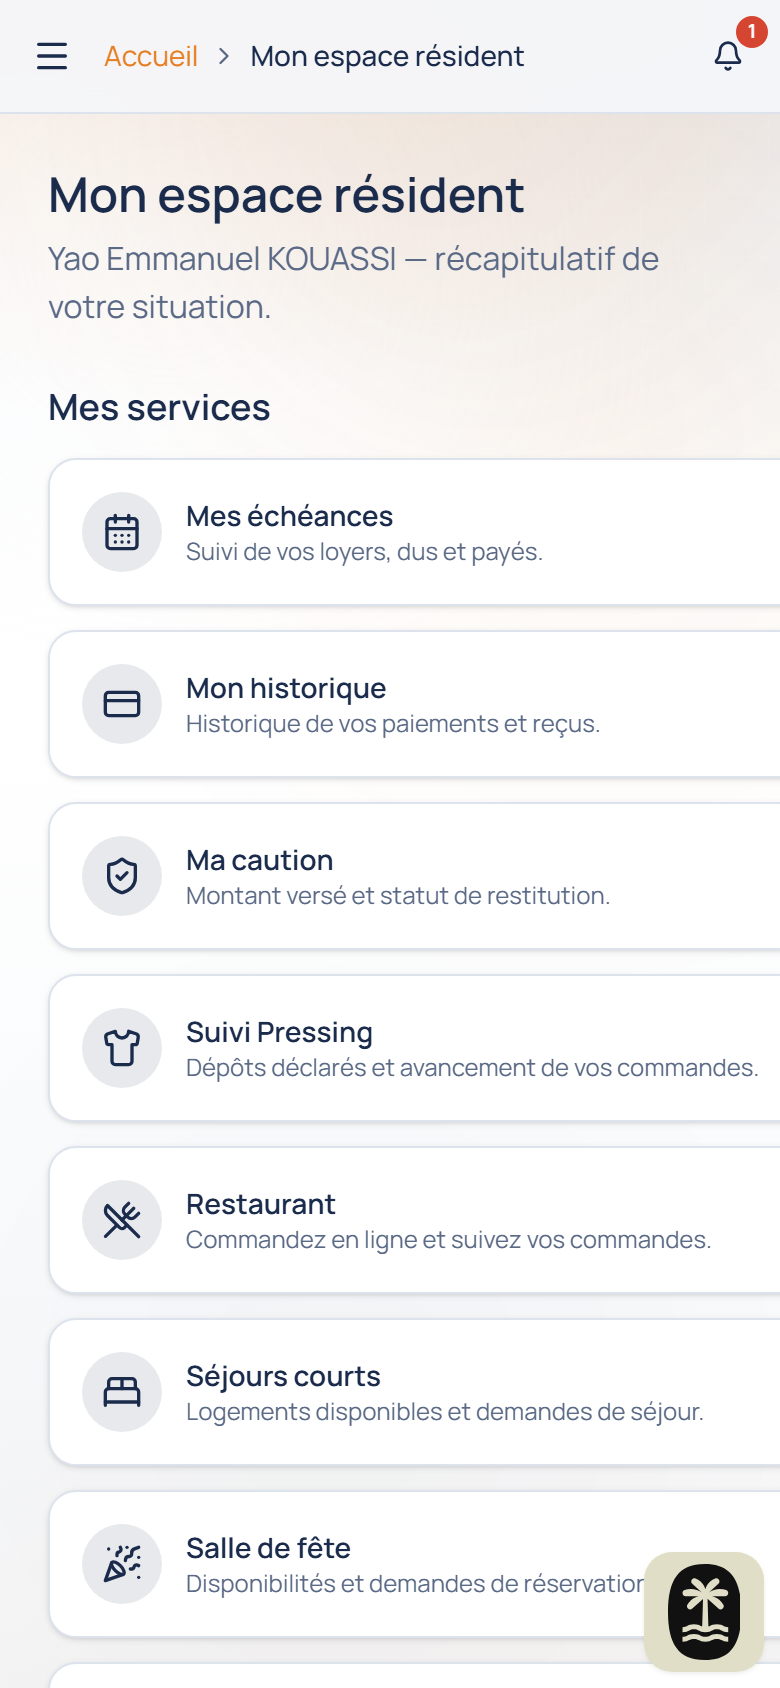
\includegraphics[width=\textwidth]{screenshots/portail/27-mobile-espace.png}
  \captionof{figure}{« Mon espace résident » sur mobile}
\end{minipage}\hfill
\begin{minipage}{0.45\textwidth}
  \centering
  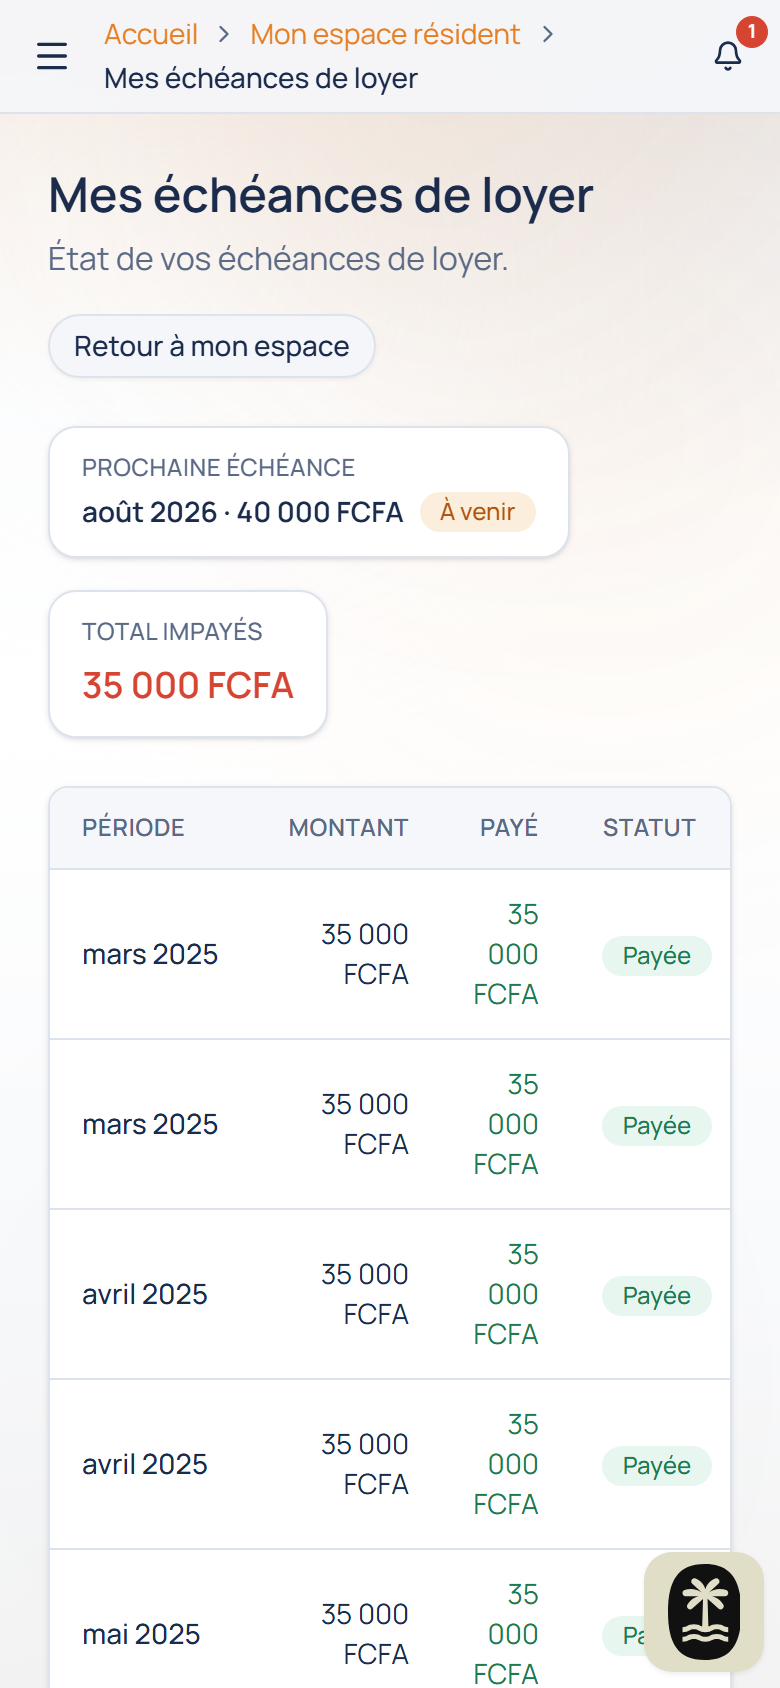
\includegraphics[width=\textwidth]{screenshots/portail/28-mobile-echeances.png}
  \captionof{figure}{Les échéances sur mobile}
\end{minipage}
\end{center}

\info{Même confort qu'à l'ordinateur : tu peux demander un séjour ou signaler un problème depuis ton lit — les photos du téléphone se joignent directement au formulaire.}

\newpage

% FAQ
\section{J'ai un problème : que faire ?}

\begin{longtable}{>{\raggedright}p{5cm} p{9cm}}
\toprule
\textbf{Problème} & \textbf{Solution} \\
\midrule
\endfirsthead
\multicolumn{2}{c}{\textit{Suite de la FAQ}} \\
\toprule
\textbf{Problème} & \textbf{Solution} \\
\midrule
\endhead
\bottomrule
\endfoot

Je n'arrive pas à me connecter & Vérifie l'identifiant et le mot de passe remis par la réception. En cas d'oubli, demande à la réception de réinitialiser ton compte. \\

La page « Mon espace résident » ne s'ouvre pas & Il te manque la permission \texttt{PORTAIL.VOIR} — demande à la réception. \\

Je ne vois pas le bouton « Passer une commande » / « Demander » & Chaque action demande sa permission (\texttt{RESTAURANT.COMMANDER}, \texttt{SALLE\_FETE.DEMANDER}…). Si le bouton manque, ton compte n'a pas le droit — demande à la réception. \\

Le reçu d'une échéance payée n'apparaît pas & Le bouton « Reçu » n'existe que sur les lignes déjà encaissées. Si tu viens de payer à la caisse, attends que le personnel enregistre le règlement. \\

Aucun logement n'apparaît dans la demande de séjour & Il n'y a pas de logement libre sur ces dates, ou les deux dates ne sont pas encore remplies. Essaie une autre période. \\

Le formulaire de séjour refuse mes dates & L'arrivée doit être dans le futur et le départ après l'arrivée — corrige les dates. \\

Un message dit que mon créneau « chevauche une réservation confirmée » & La salle est déjà prise sur cet horaire : décale l'heure ou change de date. L'encadré « Occupation du jour » te montre les jours libres. \\

Ma demande est restée « En attente de validation » & C'est normal : le personnel doit la traiter (disponibilité, tarif). Tant qu'elle est en attente, elle ne bloque ni le logement ni la salle — et tu peux l'annuler depuis sa fiche. \\

Comment annuler une demande ? & Ouvre la fiche de la demande (séjour, salle de fête, restaurant, pressing, boutique) : le bouton \textbf{Annuler la demande} est visible tant qu'elle n'a pas été validée par le personnel. \\

« Aucune photo d'état des lieux disponible » & Aucun état des lieux n'a encore été versé à ton dossier — les photos sont ajoutées par le personnel lors de la visite. \\

Je veux payer en ligne depuis le portail & Ce n'est pas prévu : tous les règlements se font sur place (réception, caisse, comptoir). Le portail sert à demander et à suivre. \\

\bottomrule
\end{longtable}

\newpage

\section{Récapitulatif des permissions}

Ce que ton compte résident peut faire dépend de ses permissions — réglées par l'administration :

\begin{itemize}[label=\textcolor{lagoon}{\faKey}]
  \item \texttt{PORTAIL.VOIR} : ouvrir le portail et voir toutes tes pages (échéances, paiements, caution, états des lieux, suivis).
  \item \texttt{RESIDENCE.DEMANDER} : envoyer une demande de séjour court et l'annuler tant qu'elle est en attente.
  \item \texttt{RESTAURANT.COMMANDER} : passer une commande au restaurant et l'annuler tant qu'elle est en attente.
  \item \texttt{SALLE\_FETE.DEMANDER} : demander une réservation de salle de fête et l'annuler tant qu'elle est en attente.
  \item \texttt{PRESSING.DECLARER} : annuler une demande de dépôt pressing encore en attente.
  \item \texttt{MARCHANDISE.COMMANDER} : demandes d'achat boutique (panier de l'espace client) et annulation tant qu'en attente.
  \item \texttt{SIGNALEMENT.VOIR} : voir tes signalements.
  \item \texttt{SIGNALEMENT.CREER} : déclarer un signalement (« Signaler un problème »).
  \item \texttt{RESIDENT.VOIR} : accéder à tes données de résident (contrat, logement).
\end{itemize}

\info{Sans la permission, le bouton correspondant n'apparaît simplement pas : ce n'est pas un bug. Demande à la réception de faire ajuster ton compte si un service te manque.}

\vfill

\begin{center}
\begin{tikzpicture}
  \node[fill=sea-ink, text=white, rounded corners=10pt, minimum width=10cm, minimum height=1.5cm, font=\large\bfseries] {Bon séjour chez GLOBAL SIM GROUP !};
\end{tikzpicture}
\end{center}

\end{document}
